\chapter{Grundlagen}
\label{Grundlagen}
In diesem Kapitel wird das Grobkonzept des Commute von Skatemate dargestellt, um einen Überblick über das Elektroskateboard zu geben. Bevor im Kapitel \ref{TechnischeGrundlagen} die dazu notwendigen Grundlagen erklärt werden, wird die Bedienung des Commute erklärt, so dass die Grundlagen besser eingeordnet werden können. 
\section{Grobkonzept}
\label{Grobkonzept}
Das Projekt Commute von Skatemate kann in drei Grundbereiche unterteilt werden: Die Steuerung über den Magic-Glove, die Motoransteuerung mittels feldorientierter Regelung FOC und die Stromversorgung mitsamt dem selbst konzipierten Akkuladegerät. Wie diese drei Bereiche miteinander interagieren ist in der Abbildung \ref{fig:grobkonzeptblockschaltbildgrob} dargestellt. Die Antriebstechnik ist über ein Kabel mit der Stromversorgung verbunden, die Inputs der Steuerung erhält sie über ein Funknetz. Nachfolgend werden die drei Bereiche detaillierter erläutert. Dargestellt sind sie im Blockschaltbild der Abbildung \ref{fig:grobkonzeptblockschaltbilddetailliert}. Zudem wird darauf eingegangen, weshalb diese Lösung gewählt wurde. 
\begin{figure}[H]
	\centering
	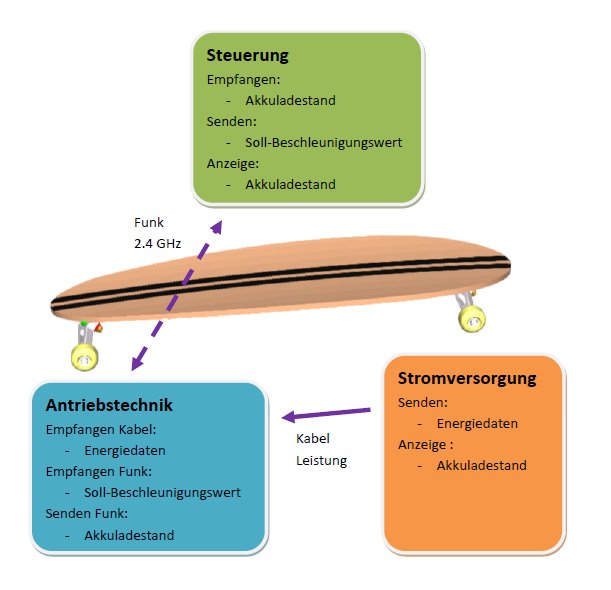
\includegraphics[width=0.7\linewidth, keepaspectratio]{images/Grobkonzept_Blockschaltbild_grob}
	\caption[Blockschaltbild Grobkonzept]{Blockschaltbild Grobkonzept}
	\label{fig:grobkonzeptblockschaltbildgrob}
\end{figure}

\subsection*{Steuerung über den Magic-Glove}
Es gibt verschiedene Wege, wie ein elektrisches Longboard gesteuert werden kann. Eine Variante ist, über Drucksensoren im Brett durch eine Gewichtsverlagerung in Fahrtrichtung eine Geschwindigkeitsregulation zu erreichen. Da auf unebenem Gelände eine natürliche Gewichtsverlagerung entsteht, und diese kompensiert werden müsste, und zudem lokal beschränkte Sensoren die Bewegungsfreiheit auf dem Longboard einschränken können, wurde diese Variante verworfen. Stattdessen wird die Geschwindigkeit über eine Fingerbewegung gesteuert. Dazu wird ein Handschuh mit integrierten Sensoren entwickelt. Dieses Wearable enthält einen Flex Sensor, der die Beugung des Zeigefinders misst. Der Flex Sensor wird im Kapitel \ref{tGl_FlexSensor} beschrieben. Die Beugung des Fingers wird mithilfe eines Mikrocontrollers quantifiziert und als Sollbeschleunigung der Motoransteuerung übergeben. Dies geschieht über ein 2.4 GHz Funknetz, dazu ist ein Funkmodul integriert. Die Stromversorgung erfolgt über eine Li-Ion Knopfbatterie LTR2450. 
In der Abbildung \ref{fig:grobkonzeptblockschaltbilddetailliert} sind die einzelnen Elemente der Steuerung dargestellt.

\subsection*{Antriebstechnik}
Als Antrieb ist der OX1 2-10 Motor vorgegeben, dies ist ein Brushless-Gleichstrommotor (BLDC-Motor). Er verfügt nicht über Hallsensoren. Die technischen Hintergründe des Motors werden im Kapitel \ref{tGl_BLDC} gegeben. Ein BLDC-Motor ist wie ein permanentmagnetischer Drehstrom-Synchronmotor (PMSM) aufgebaut.\\
Die Ansteuerung kann über eine Kommutierung oder eine Vektorregelung erfolgen\cite{BLDC} \todo{[ Quelle xxx ]}. Die Kommutierung kann prinzipiell gesteuert oder ungesteuert erfolgen. Bei der ungesteuerten Kommutierung kann der Motor als Schrittmotor genutzt werden, die Rotorposition folgt der Steuerung. Diese Variante ist für ein gleichmässig rollendes Longboard ungeeignet. Die Kommutierung muss also abhängig von der Rotorposition erfolgen (geführte Kommutierung), die Steuerung reagiert also auf die effektive Rotorposition und passt sich dieser an.\todo{(xxx korrekt?} Am einfachsten wäre diese mit Sensoren, da unser Motor jedoch nicht über Sensoren verfügt, muss der Motor über eine sensorlose gesteuerte Kommutierung angesteuert werden. Dies funktioniert jedoch nur ab einer Mindestdrehzahl wirklich gut. Zum Anfahren muss der Motor speziell angesteuert werden. \\
Bei der Vektorreglung, in diesem Fall eine Feldorientierte Regelung (field oriented controll, FOC), werden die Spannungen zur Steuerung aktiv der Rotorlage angepasst. Auch mit der FOC kann zwischen sensorgesteuerte und sensorlosen Regelung unterschieden werden. Bei der sensorlosen Regelung muss wiederum zum Anfahren eine zusätzliche Ansteuerung erfolgen. \todo{Diese wird im Kapitel xxx erklärt.} Kann die Anfangsposition jedoch genügen genau geschätzt werden, läuft der Motor auch bei tiefen Geschwindigkeiten gleichmässig, da er genauer geregelt werden kann. Dies entspricht unseren Anforderungen für das Commute, da ein sanftes Anfahren sehr wichtig ist. Die FOC ist im Kapitel \ref{tGl_FOC} erklärt.\\
Ausgeführt wird die FOC auf einem Mikrocontroller. Mittels eines RF-Modul wird die Sollbeschleunigung empfangen. Eine Halbbrücke mit FET-Treibern (siehe Kapitel \ref{tGl_HBrugg}) setzt  die gewünschte Motorsteuerung um. Zur Übersicht sind diese Elemente im Blockschaltbild Abbildung \ref{fig:grobkonzeptblockschaltbilddetailliert} dargestellt. 

\begin{figure}[h]
	\centering
	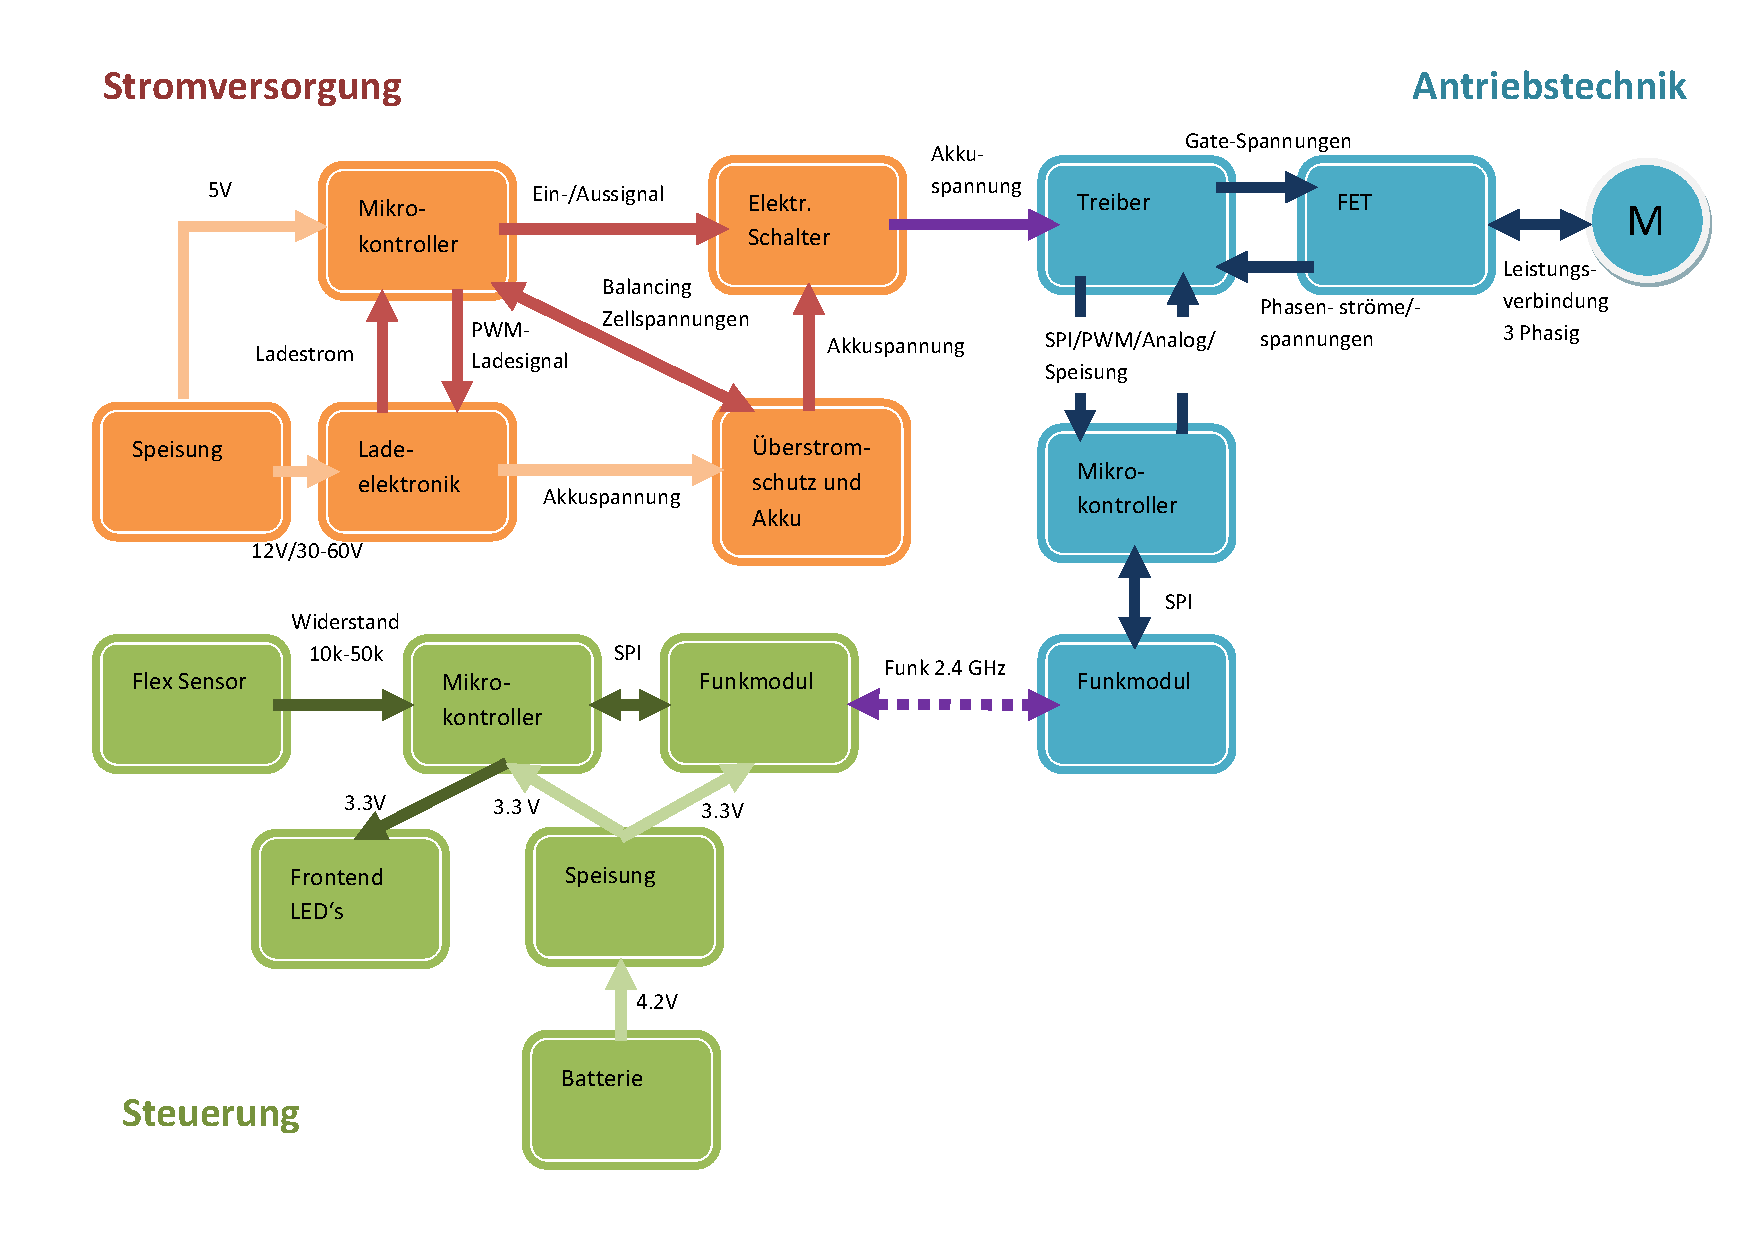
\includegraphics[width=\linewidth]{images/Grobkonzept_Blockschaltbild_detailliert}
	\caption[Detailliertes Blockschaltbild]{Detailliertes Blockschaltbild}
	\label{fig:grobkonzeptblockschaltbilddetailliert}
\end{figure}

\subsection*{Stromversorgung}
Die Stromversorgung erfolgt über ein LiPo 5200mAh Akku, dieser ist vorgegeben. Es besteht ein externes Ladegerät. Da dies jedoch bedeutet, dass der Akku für jedes Laden vom Longboard gelöst werden muss. Dies ist umständlich und gefährdet die Wetterfestigkeit und Robustheit des Commute. Deshalb wird ein eigener, integrierter Akkulader entwickelt, so dass der Akku nicht mehr herausgelöst werden muss. Da die Entladung im Gebrauch sowieso überwacht werden muss, ist der Lader eine Ergänzung und kein alleinstehendes Element. Kernstück der Stromversorgung ist die Balancerschaltung. Dabei wird der Akku erst mit einem konstanten Strom geladen, bis die Zellspannung erreicht ist. Anschliessend wird mit einer konstanten Spannung geladen, bis der Strom unter 100mA gesunken ist, dann sind die Zellen vollständig geladen. Wie das Balancing genau funktioniert, ist im Kapitel \ref{tGl_Balancing} beschrieben. Anstelle einer eigenen Implementation hätte ein fertiges IC eingekauft werden können, aus finanziellen Gründen wurde jedoch darauf verzichtet. Die Elemente der Stromversorgung sind in der Abbildung \ref{fig:grobkonzeptblockschaltbilddetailliert} dargestellt.

\section{Bedienung}
Im folgenden wird die Bedienung des Commute beschrieben. Dabei wird erst die Inbetriebnahme beschrieben, anschliessend der alltägliche Gebrauch und zuletzt wird erklärt, wie der Akku geladen werden kann.
\subsection*{Erste Inbetriebnahme}
Bei der ersten Inbetriebnahme des Commute muss der Magic-Glove kalibriert werden. Insbesondere wird dabei die Ruhestellung der Hand definiert. Der Nutzer drückt drei Sekunden auf den Taster, dann zeigen die LEDs die Ruhestellung an, das heisst, alle leuchten und diese in der Mitte leuchten am stärksten. Nun hält der Nutzer seine Hand in Ruhestellung, also so wie er gerne auf dem Longboard steht. Dies wird als Nullposition definiert. Anschliessend beginnen die LEDs zu laufen – in eine Richtung führt der Nutzer dazu eine Bremsbewegung aus, in die andere Richtung die Bewegung, um zu Beschleunigen. Anschliessend ist die Kalibration abgeschlossen. Nun kann das Commute genutzt werden.
\subsection*{Alltägliche Handhabung}
Auf dem Longboard befindet sich ein on/off-Schalter, ebenso auf dem Magic-Glove. Werden diese angeschaltet, ist das Commute betriebsbereit und der Nutzer kann losfahren. 
Entfernt sich der Nutzer mehr als drei bis vier Meter vom Bord, ist die Kommunikationsverbindung zwischen der Steuerung und der Antriebstechnik unterbrochen, und das Commute schaltet sich automatisch aus. Während der Fahrt wird dem Nutzer mithilfe der LEDs der Batteriestand des LiPo-Akkus angezeigt. Zudem wird die Batterie des Magic-Gloves überwacht und auch über die LEDs angezeigt. 
\subsection*{Akku aufladen}
Der Akku kann praktisch über einen Stecker am Longboard aufgeladen werden, der Akku muss also nicht herausgelöst werden. Während dem Ladevorgang zeigen drei LEDs am Longboard den Ladestand an. Diese LEDs leuchten auch kurz auf, wenn das Longboard eingeschaltet wird und zeigen damit den Akkustand. 


%\todo{cite rausnehmen}
%TEST\\
%\cite{test}
%\\TEST\\
%\cite{testBuch}